\subsection{Surface inspection using an Atomic Force Microscope}
\textit{Atomic Force Microscopy} (AFM) is a sophisticated type of 
scanning probe microscopy, which consists of a physical probe
that scans the specimen in order to produce images of surfaces. 
Atomic Force Microscopes can map the topology of a surface
with sub-nanometric resolution, which makes them an ideal tool 
for surface inspection in the context of atomic sensors, and
more specifically in the context of Optical Contact Bonding,
due to the strict glass roughness requirements of this method. 
\\\\
The AFM consists of a cantilever with a sharp tip at 
its end ---with a radius of curvature 
on the order of nanometers, as shown in \ref{fig:AFM_tip}--- that is used to scan 
the specimen surface. 
When the tip is brought near a sample, forces between them lead to a 
deflection of the cantilever according to Hooke's law. Forces that 
are measured in AFM include mechanical 
contact force, van der Waals forces and capillary forces, among others.
Operating modes are  divided into static \textit{contact} modes and \textit{tapping}
modes, where the cantilever is vibrated at a given frequency.
\begin{figure}[h]
    \centering
    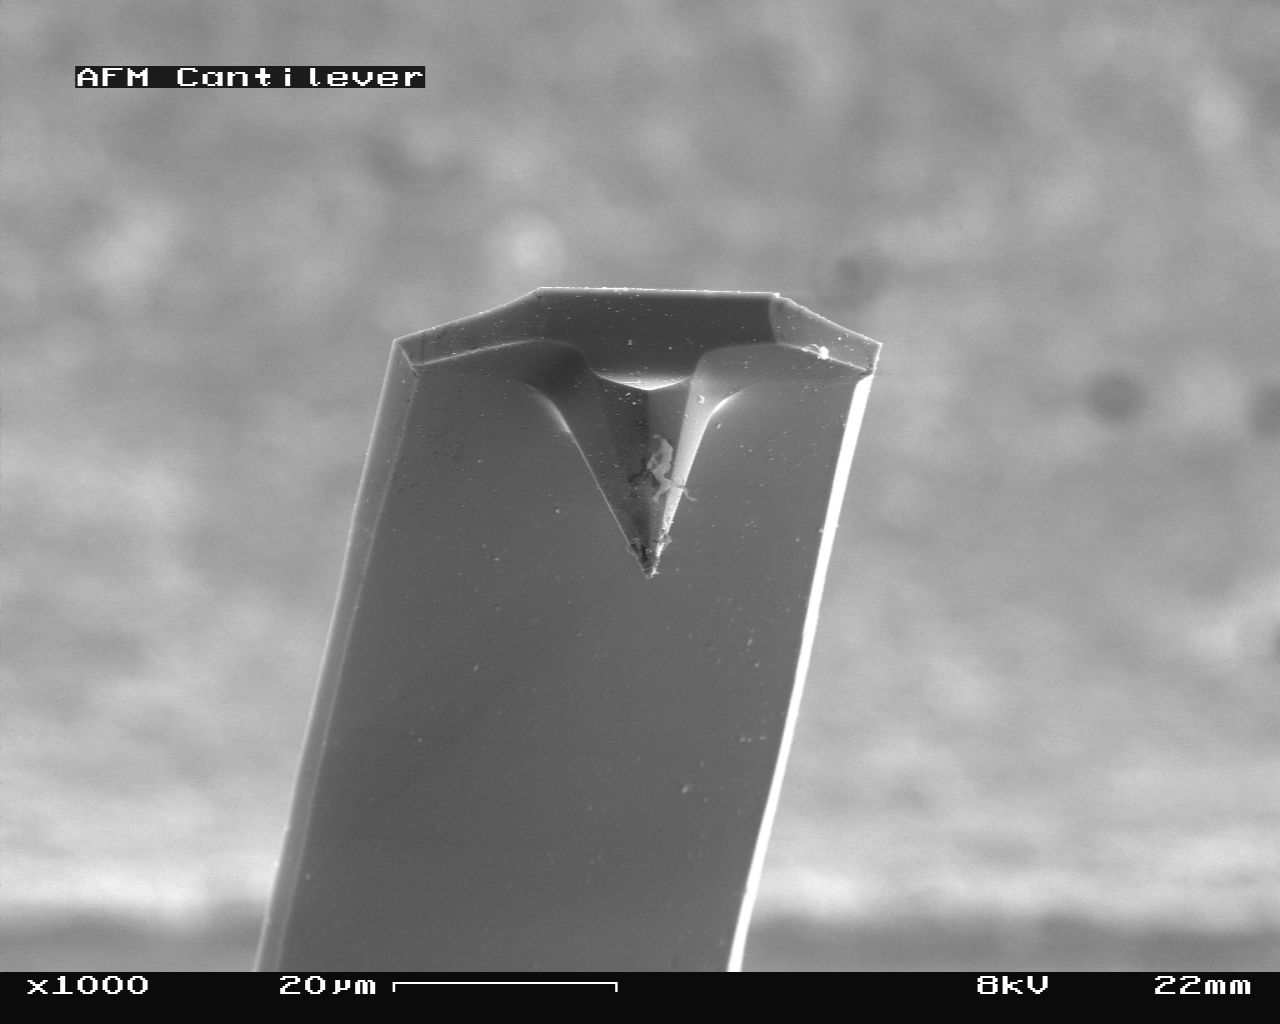
\includegraphics[width=0.6\linewidth]{Images/AFM_tip.JPG}
    \caption{View of cantilever in Atomic Force Microscope (magnification 1000x) \cite{wiki_afm_tip}}
    \label{fig:AFM_tip}
\end{figure}
\\\\
A brand-new Nanoquartz glass disk, with specified Root Mean Square roughness
of \SI{500}{\pico\meter} and Total Thickness Variation (TTV) of \SI{2}{\micro\meter} 
was inspected using a Park NX10 AFM, with a tip Park Scout 350 in \textit{tapping} mode 
(resonance frequency \SI{320}{\kilo\hertz}, rate \SI{0.5}{\hertz}).
It was examined in three different spots of its surface. The obtained data was analyzed
using the \textit{Gwyddion} software, where 
two \ref{fig:AFM_image2D} and three-dimensional \ref{fig:AFM_image3D}
AFM images of the samples were obtained,
along with the density distribution of roughness ---displayed in 
\ref{fig:roughness_dist}. A detailed list of the estimated
surface parameters can be found in \ref{tab:afm}. The precise definition of these parameters 
can be found in \cite{ISO}. 
\begin{figure}
    \centering
    \begin{subfigure}[b]{0.55\textwidth}
        \includegraphics[width=\textwidth]{Images/Sample1_2D_compressed.pdf}
    \end{subfigure}
    \vfill
    \begin{subfigure}[b]{0.48\textwidth}
        \includegraphics[width=\textwidth]{Images/Sample2_2D_compressed.pdf}
    \end{subfigure}
    \begin{subfigure}[b]{0.48\textwidth}
        \includegraphics[width=\textwidth]{Images/Sample3_2D_compressed.pdf}
    \end{subfigure}
    \caption{2D Surface images obtained through AFM in three different
    parts of the pristine Nanoquartz disk's surface.}
    \label{fig:AFM_image2D}
\end{figure}
\begin{figure}
    \centering
    \begin{subfigure}[b]{0.48\textwidth}
        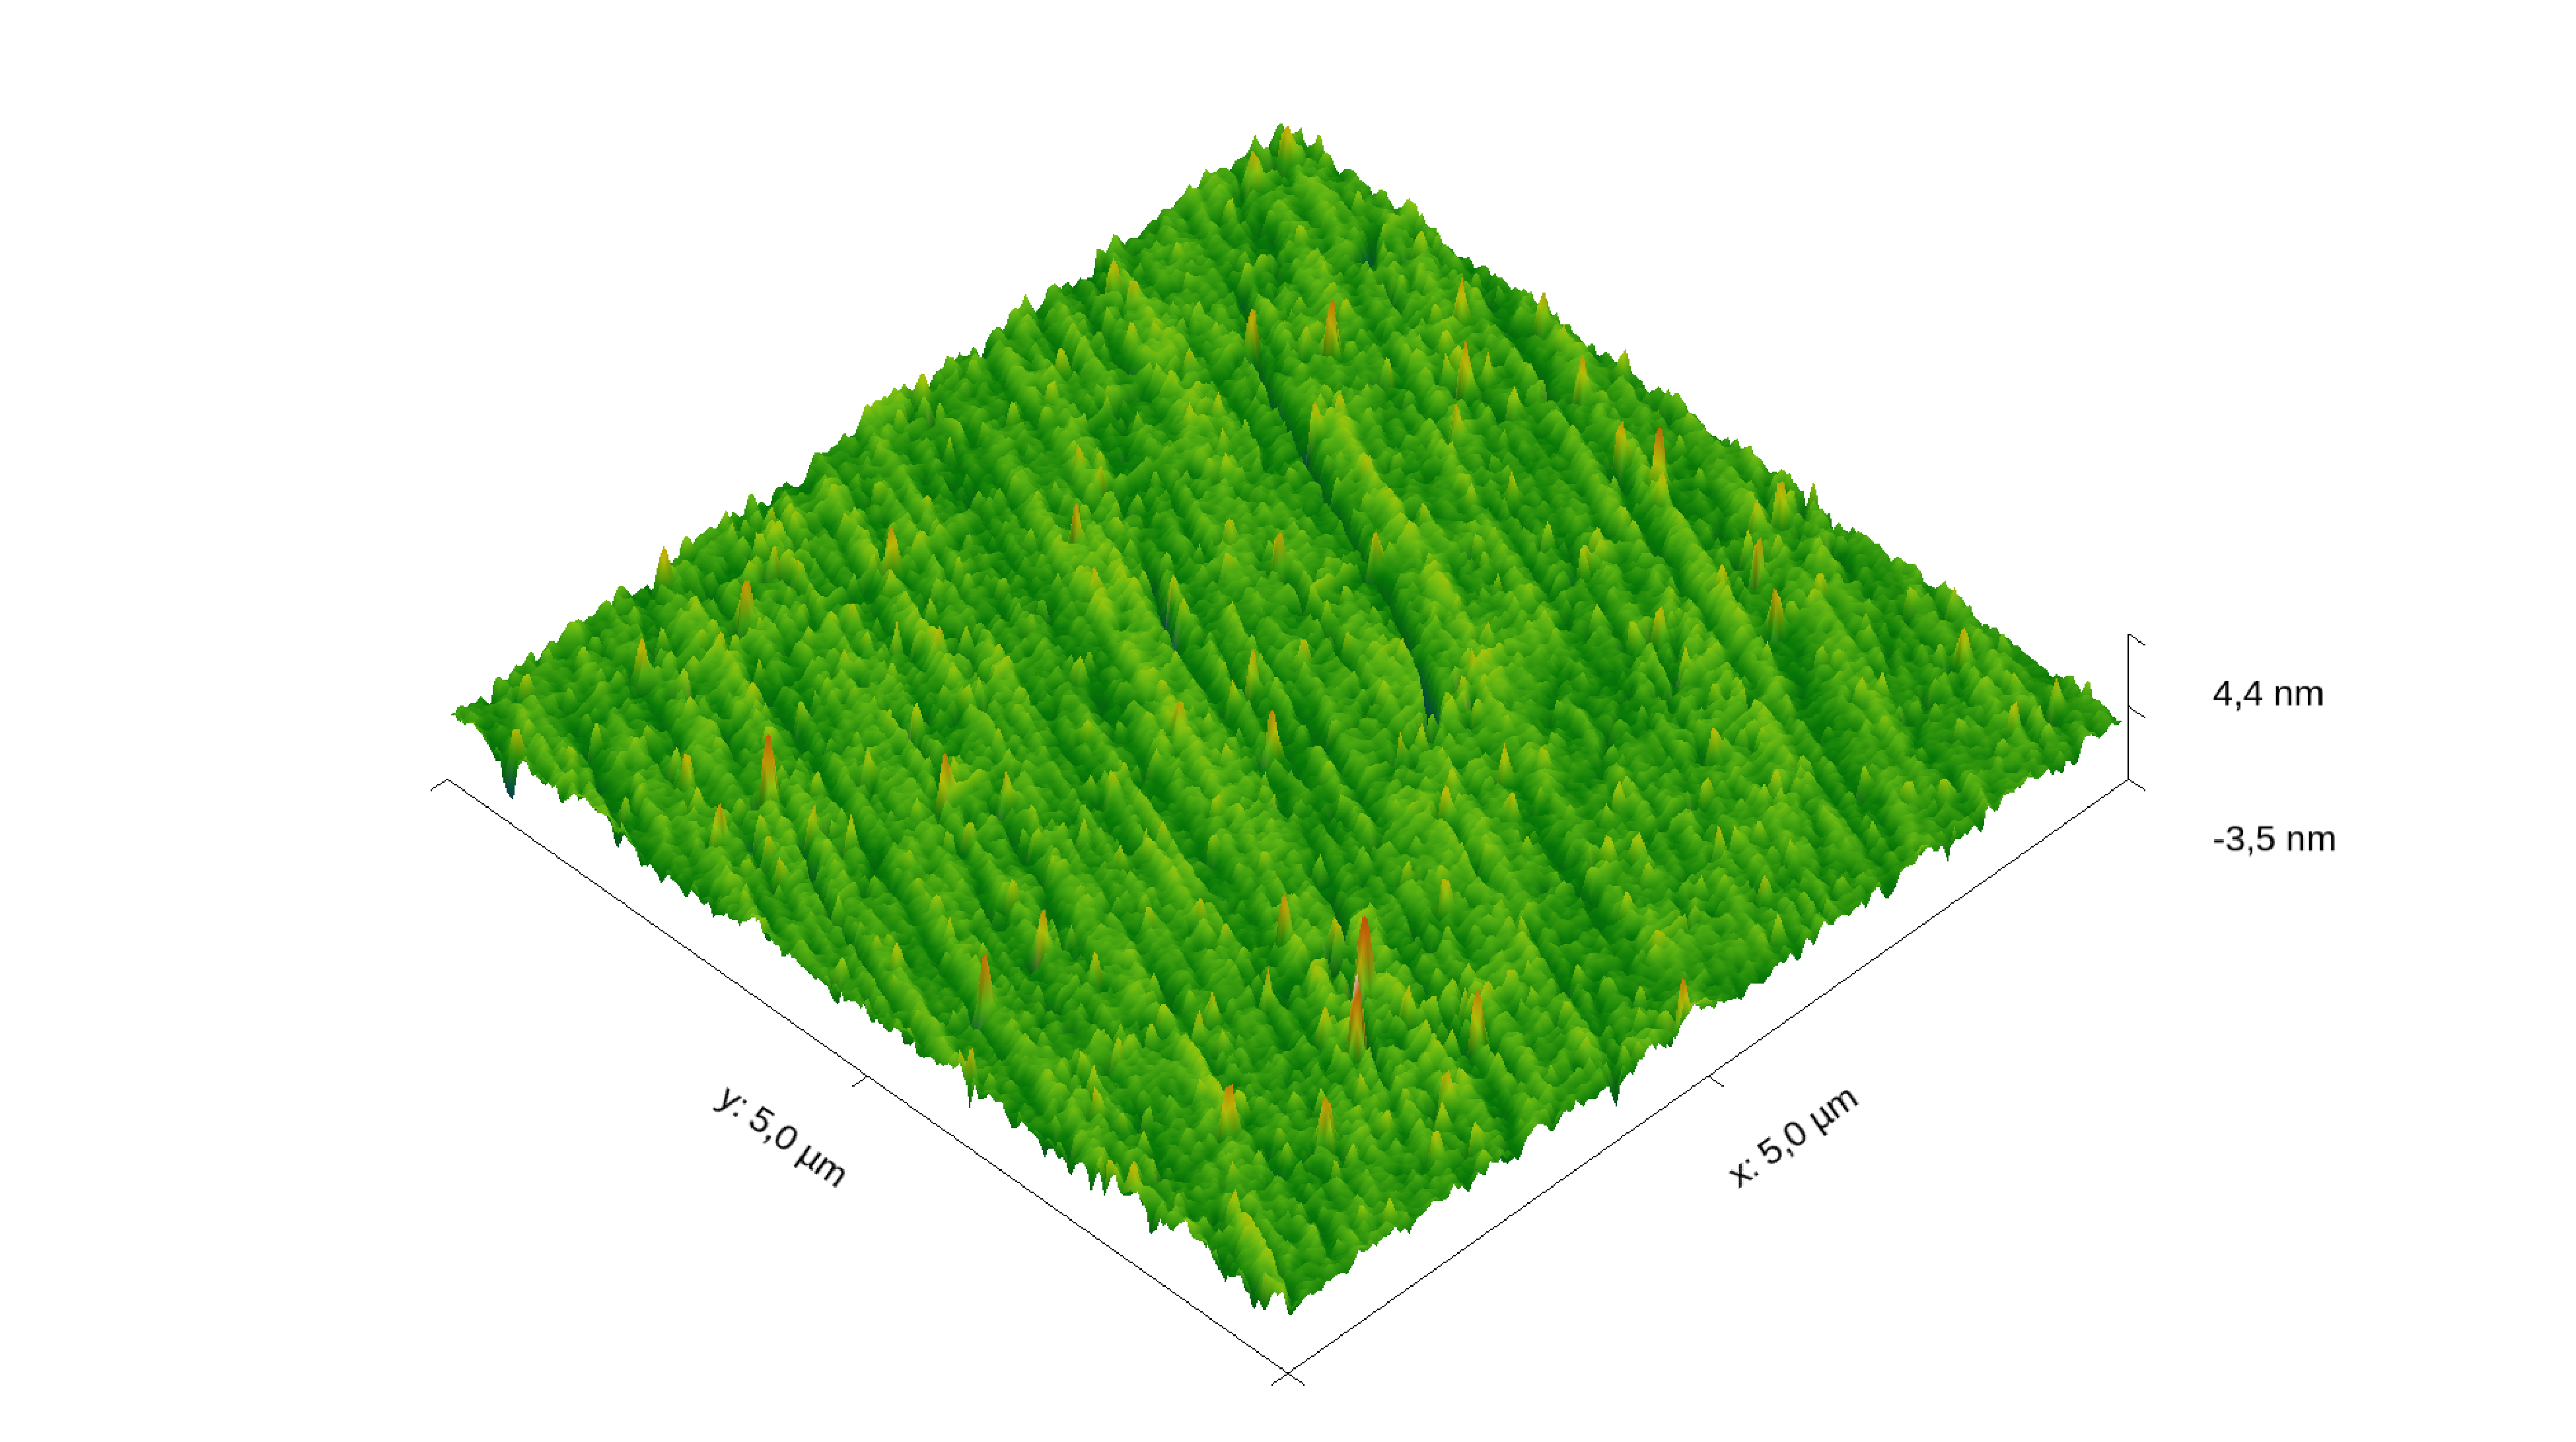
\includegraphics[width=\textwidth]{Images/Sample1_3D.pdf}
    \end{subfigure}
    \vfill
    \begin{subfigure}[b]{0.48\textwidth}
        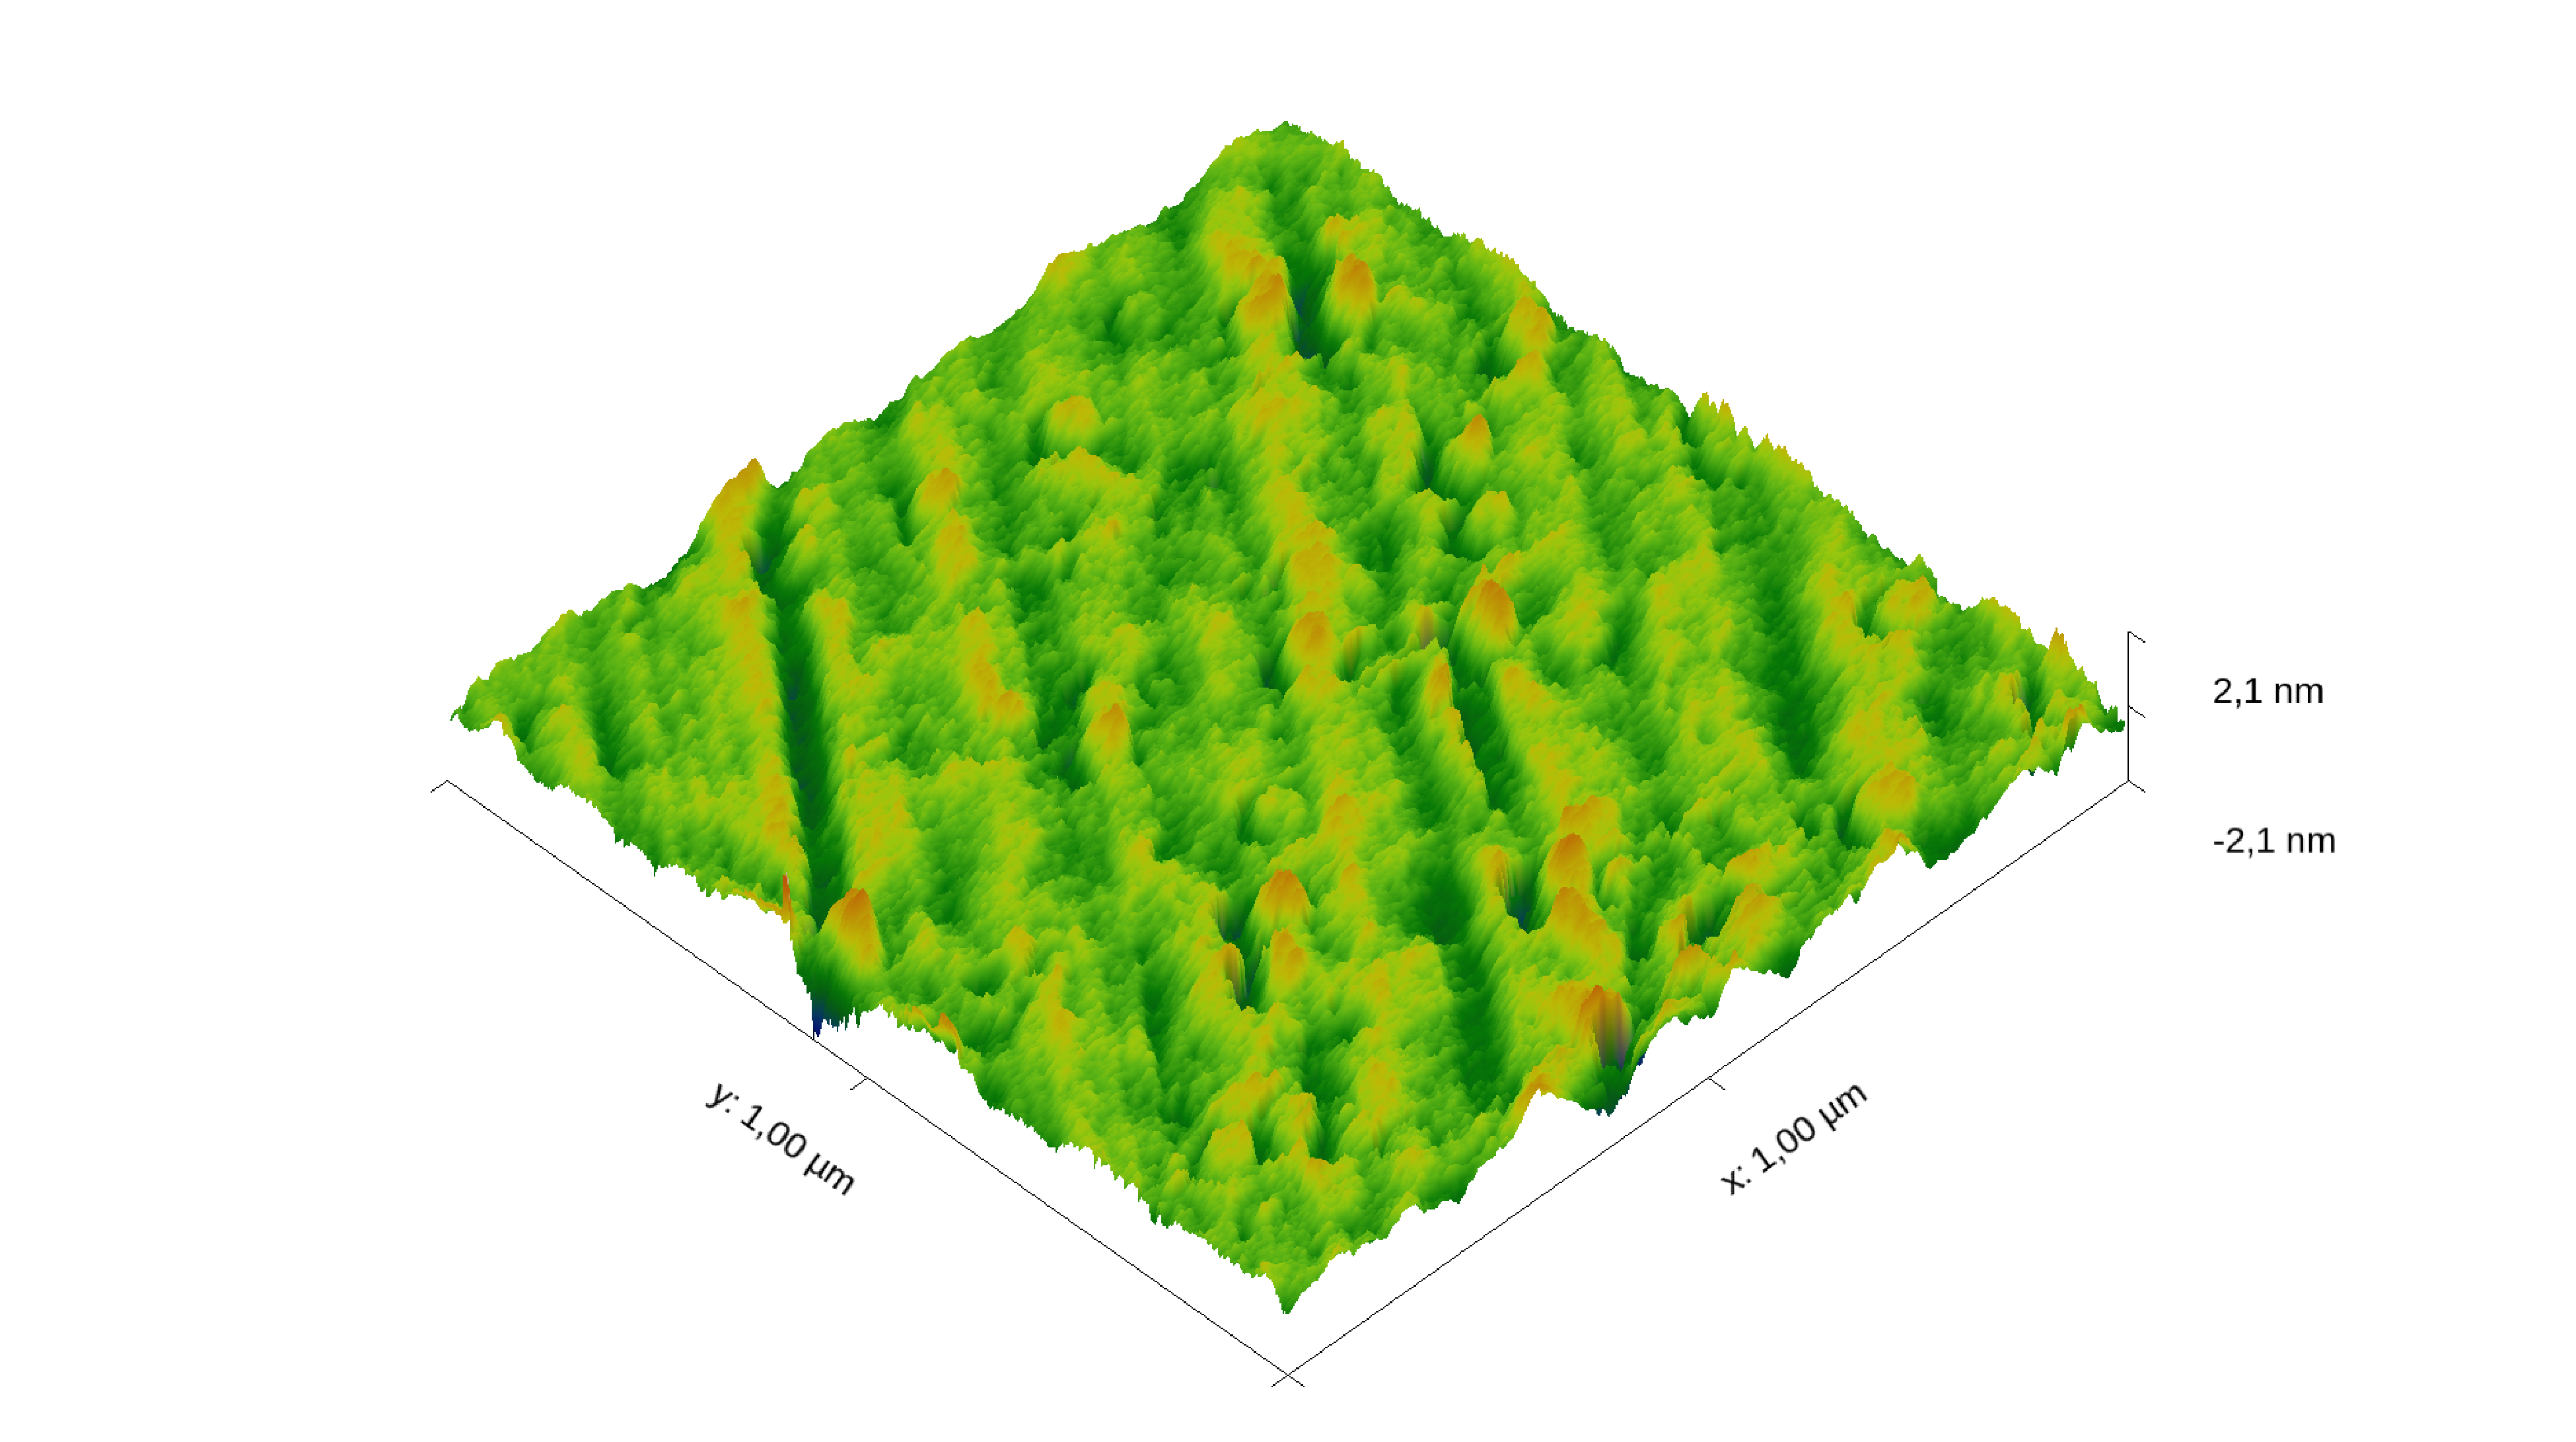
\includegraphics[width=\textwidth]{Images/Sample2_3D.pdf}
    \end{subfigure}
    \begin{subfigure}[b]{0.48\textwidth}
        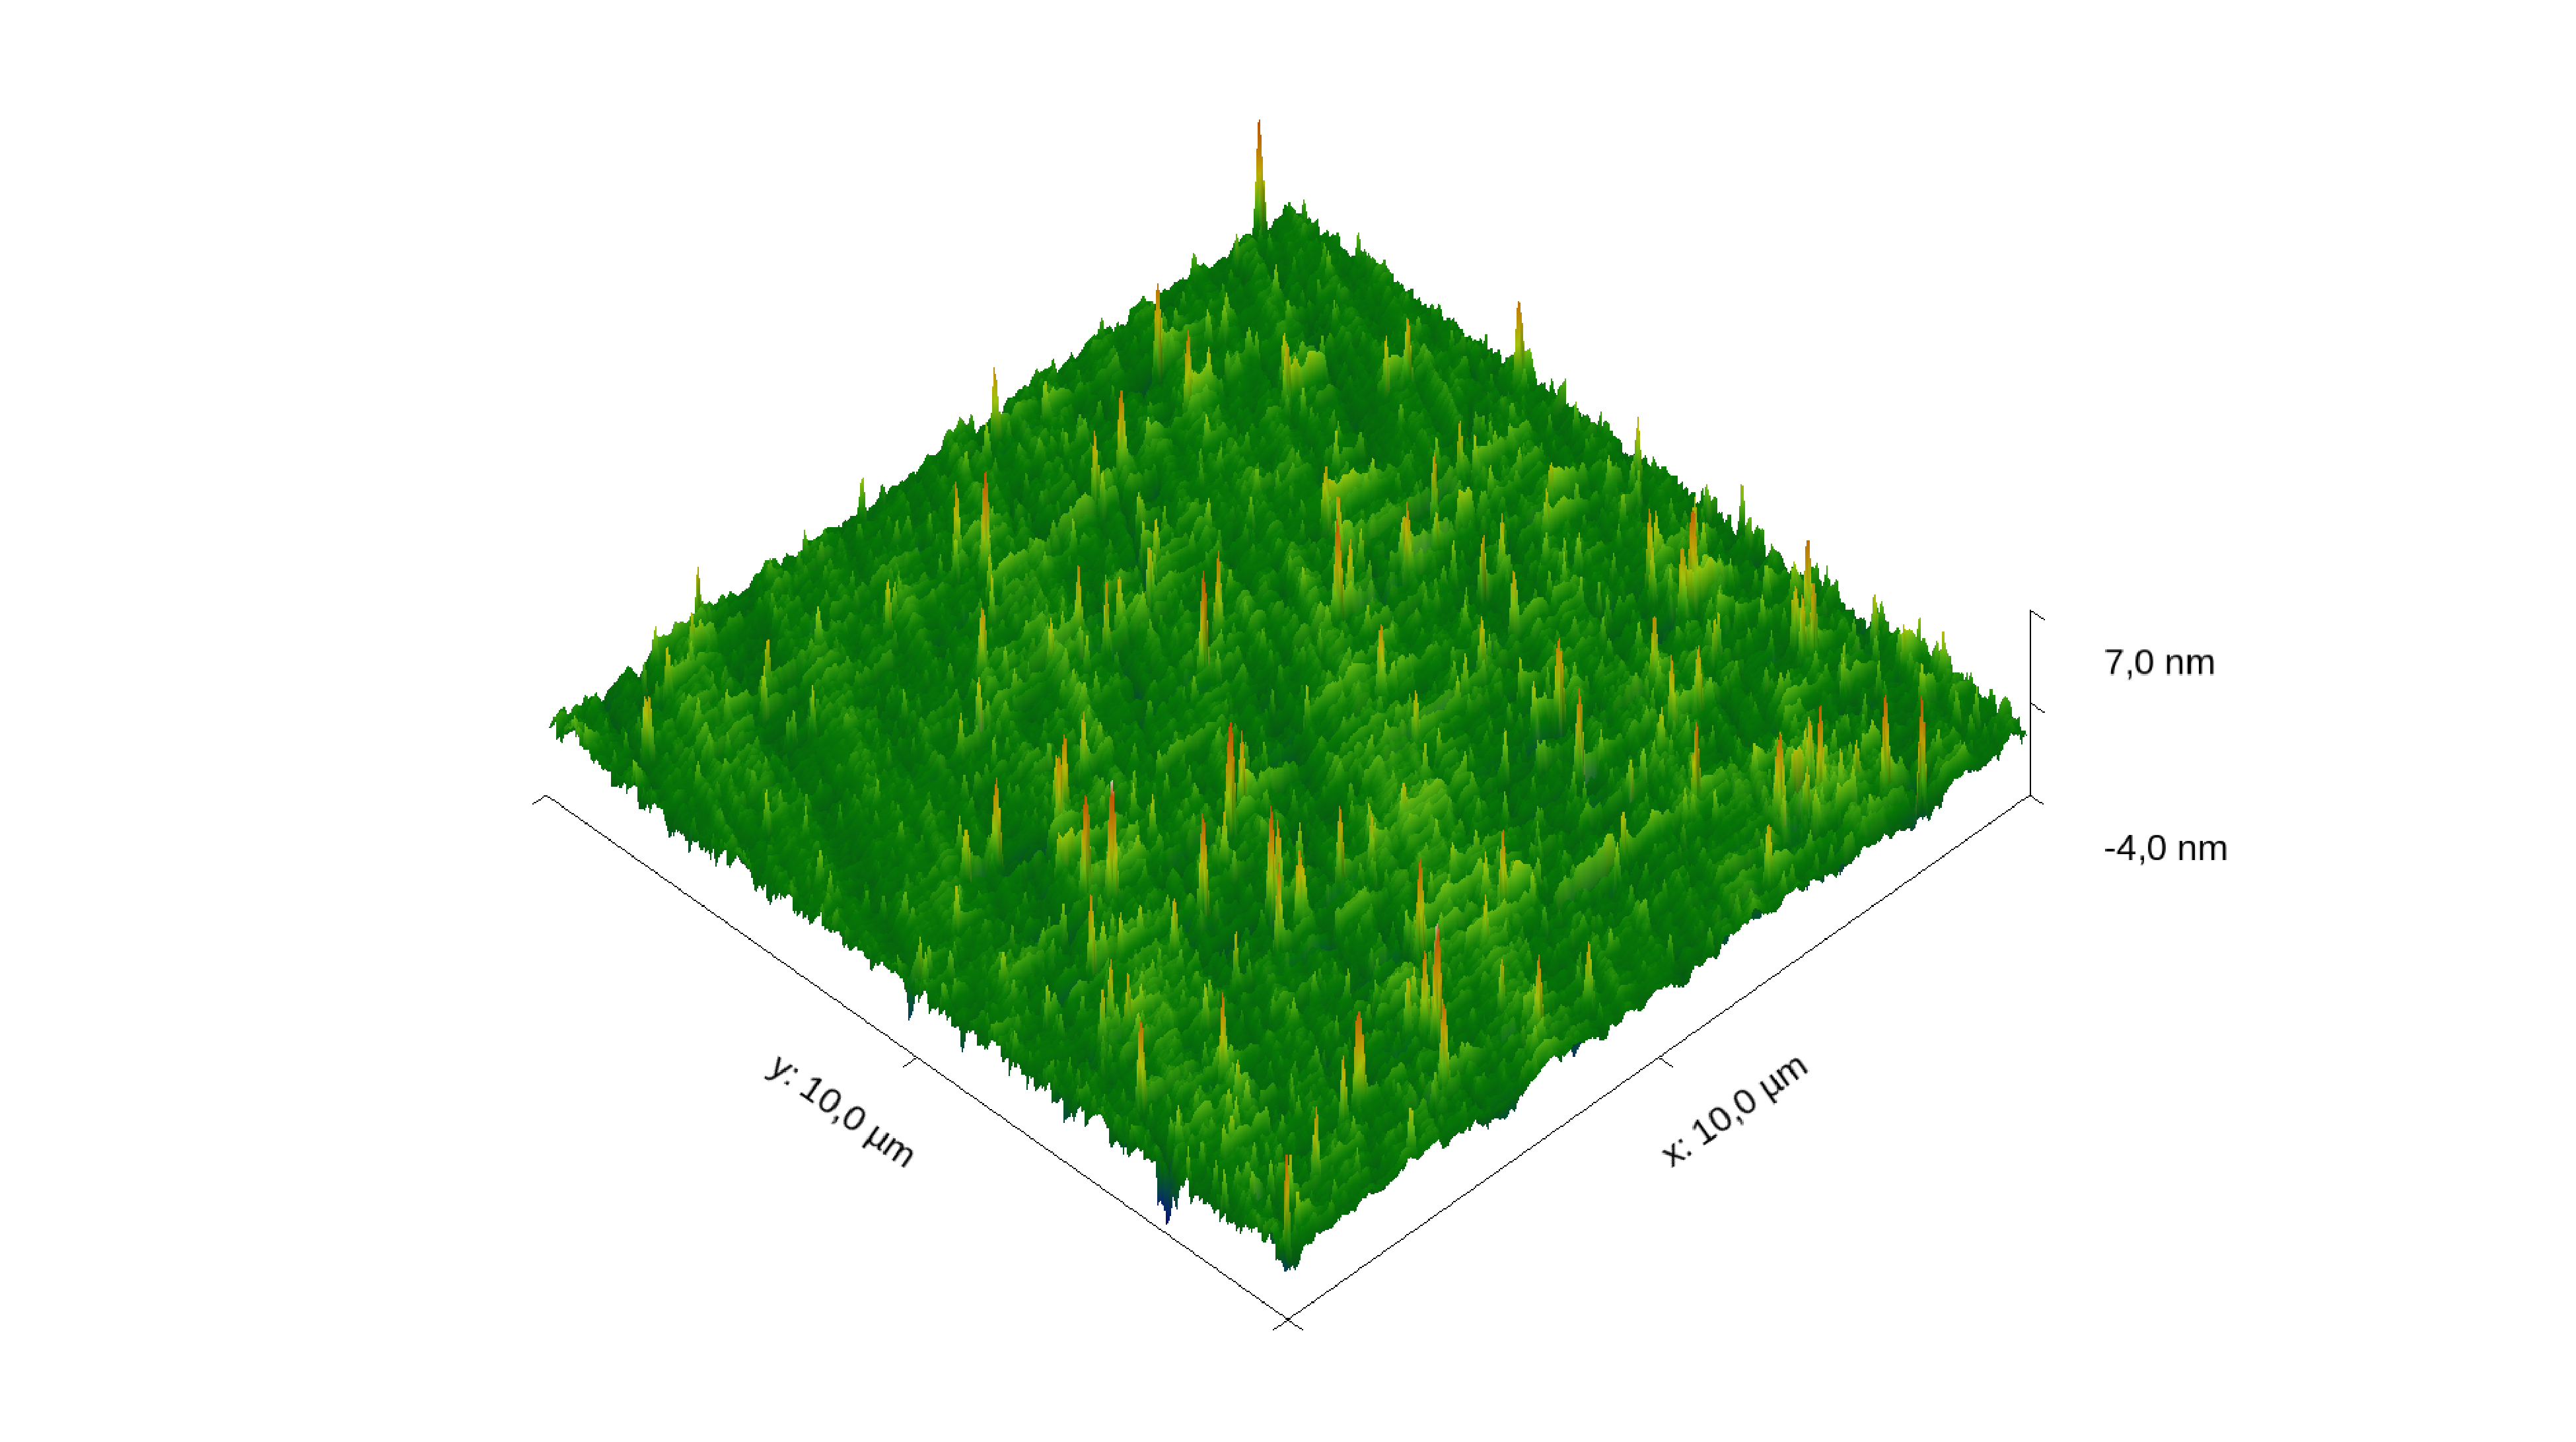
\includegraphics[width=\textwidth]{Images/Sample3_3D.pdf}
    \end{subfigure}
    \caption{3D Surface images obtained through AFM in three different
    parts of the pristine Nanoquartz disk's surface.}
    \label{fig:AFM_image3D}
\end{figure}
\begin{figure}
    \centering
    \begin{subfigure}[b]{0.48\textwidth}
        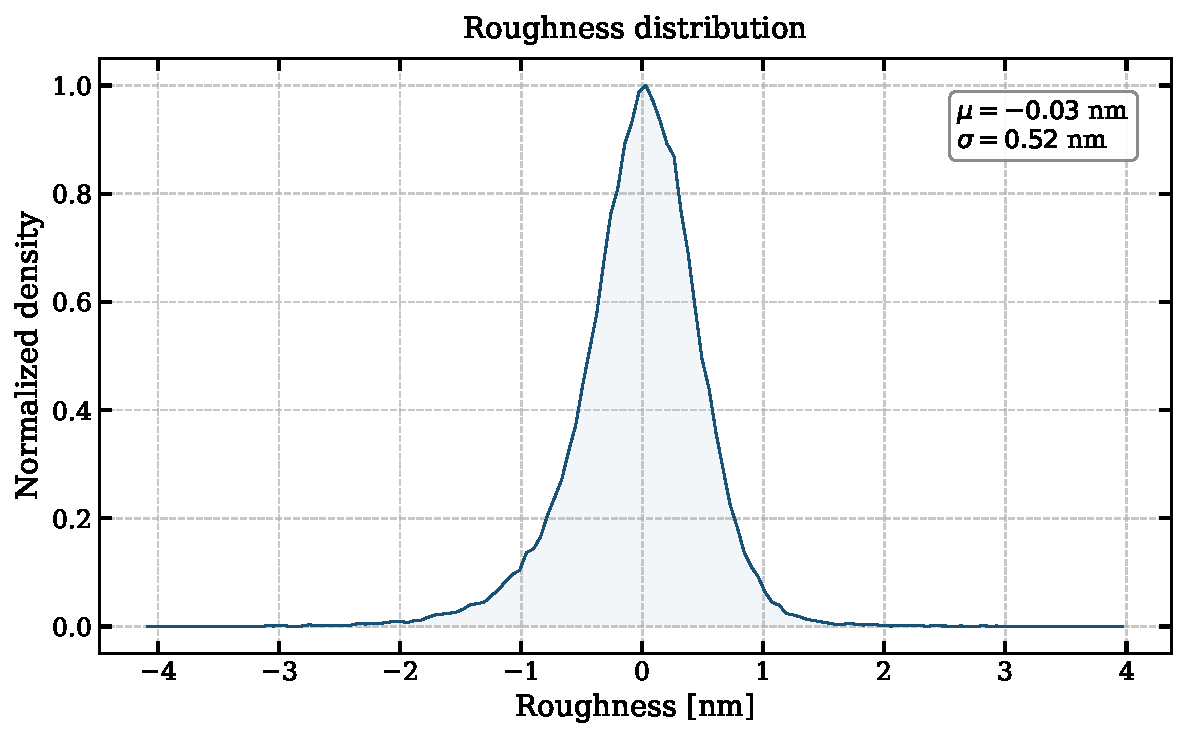
\includegraphics[width=\textwidth]{Images/Sample1_dist.pdf}
    \end{subfigure}
    \vfill
    \begin{subfigure}[b]{0.48\textwidth}
        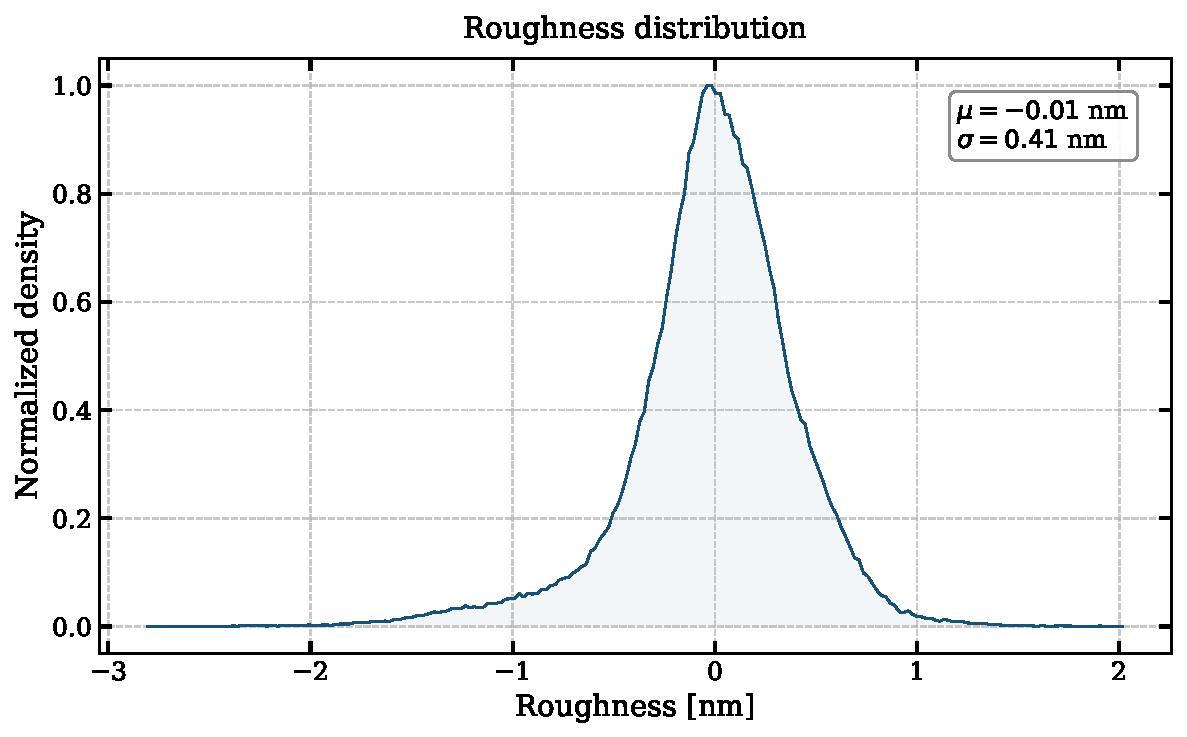
\includegraphics[width=\textwidth]{Images/Sample2_dist.pdf}
    \end{subfigure}
    \begin{subfigure}[b]{0.48\textwidth}
        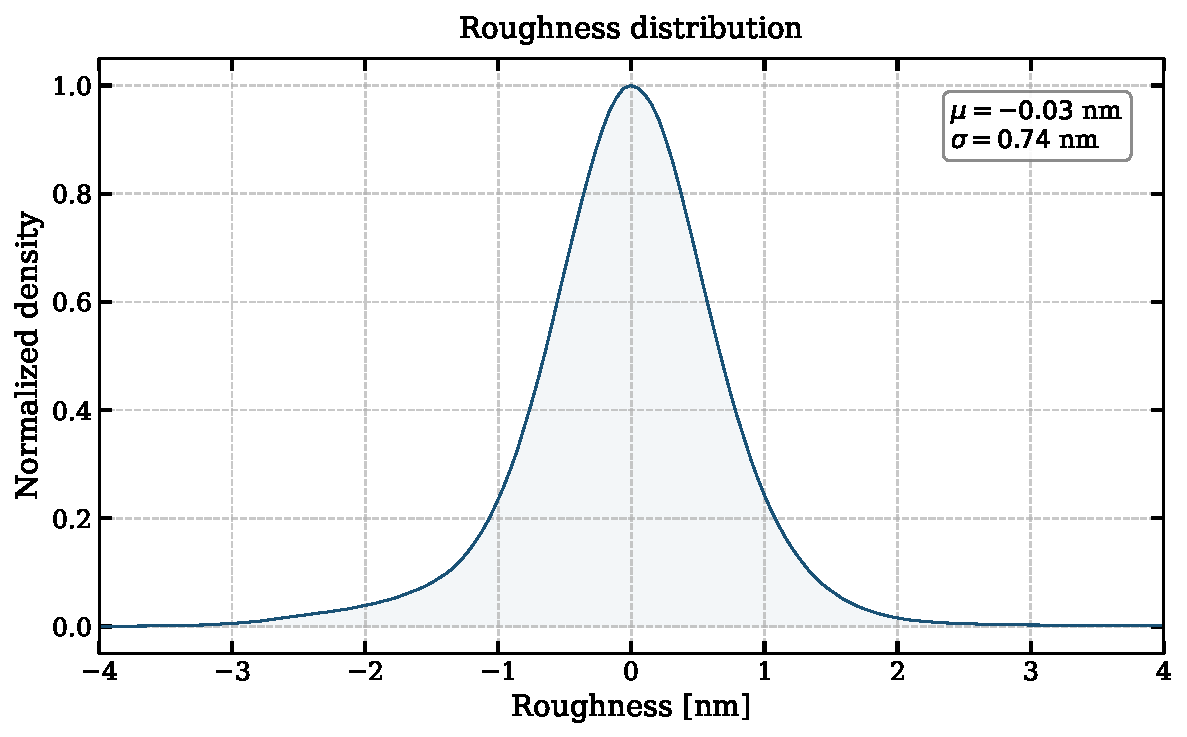
\includegraphics[width=\textwidth]{Images/Sample3_dist.pdf}
    \end{subfigure}
    \caption{Surface roughness distribution obtained through AFM. It can be seen
    that most of the defects are below the \SI{1}{\nano\meter} range. Furthermore,
    the mean ($\mu$) is close to zero, confirming that the surface is uniform.}
    \label{fig:roughness_dist}
\end{figure}
\begin{table}[h]
\centering
\resizebox{\textwidth}{!}{%
\begin{tabular}{l|l|l|l|l|l|l}
\textbf{Sample} & \textbf{$S_q$ {[}pm{]}} & \textbf{$S_a$ {[}pm{]}} & \textbf{$S_p$ {[}nm{]}} & \textbf{$S_v$ {[}nm{]}} & \textbf{$S_z$ {[}nm{]}} & \textbf{Mean height {[}nm{]}} \\ \hline
\textbf{1}      & 518                  & 387                  & 4.02                 & -4.14                & 8.17                 & 0.03                          \\ \hline
\textbf{2}      & 411                  & 298                  & 2.04                 & 2.83                 & 4.87                 & 0.02                          \\ \hline
\textbf{3}      & 726                  & 529                  & 7.66                 & 4.05                 & 11.71                & 0.02                         
\end{tabular}%
}
\caption{Surface parameters obtained through AFM in three different parts of the surface:
\textit{Root mean square roughness} ($S_q$),
 \textit{Mean roughness} ($S_a$), \textit{Maximum peak height} ($S_p$),
 \textit{Minimum valley depth} ($S_v$), \textit{Maximum height} ($S_z$)
 and \textit{Mean height}}
\label{tab:afm}
\end{table}
\\\\
The results confirm that the Root Mean Square roughness of the disk is around \SI{500}{\pico\meter},
as suggested by the manufacturer. An alternative estimation of the surface roughness,
known as \textit{Mean roughness} (Sa) was found to be in the same order of magnitude.
Additionally, it was determined that the total height ($S_q$)
is in the range of a few nanometers. The mean height is approximately zero, 
suggesting that the surface's defects are uniformly distributed. The outstanding surface parameters
observed in this disk comply with Optical Contact Bonding requirements and therefore it is suitable 
for the fabrication of Laser-Written Vapor Cells and high-precission atomic sensors.  